\section{Project structure}

Any \ESCRIBA project will generate the structure depicted by figure
\ref{fig:project_layout}.

\begin{figure}[h]
  \centering
  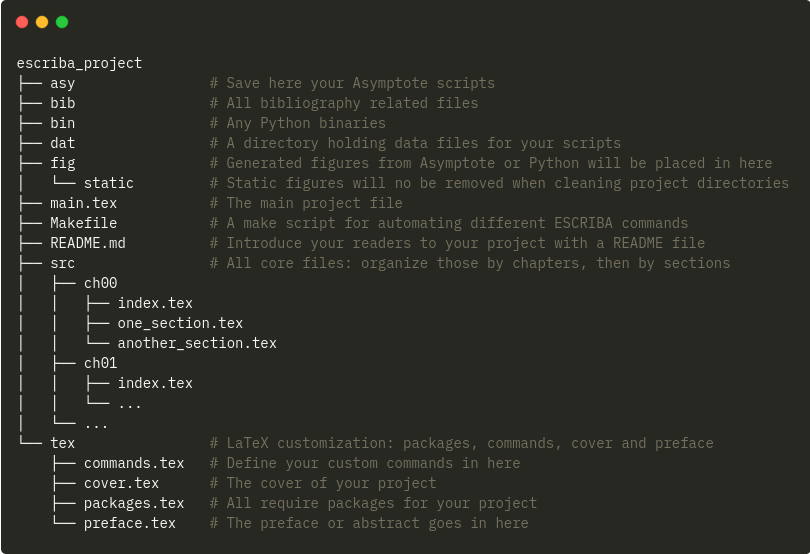
\includegraphics[width=\linewidth]{static/project_layout.png}
  \caption{Generic ESCRIBA project layout.}
  \label{fig:project_layout}
\end{figure}

Each one of the directories is devoted to a particular task:

\begin{itemize}

  \item The main goal of the asy/ directory is to store all the
        \href{https://asymptote.sourceforge.io/}{Asymptote} scripts for generating the different
        vector figures of your project. \ESCRIBA will automatically detect if
        any figure is present, compile it and move it temporary to the fig/
        folder before compiling your \LaTeX document.

  \item The bib/ directory is expected to store all the bibliography files,
        who's extension is *.bib. You will need to link manually those in the
        main.tex file.

  \item Regarding the bin/ folder, it is devoted to the storage of binaries.
        These can be Python files or any other ones. However, for the moment,
        \ESCRIBA is only expected to work with Python scrips.

  \item The dat/ directory can be used to save different data files used by the
        binaries.

  \item For the fig/ folder, every PNG file which is not stored in the
        fig/static/ directory will be assumed to be a temporary file. This is
        because the output of the
        \href{https://asymptote.sourceforge.io/}{Asymptote} scripts or the
        figures developed using the Python binaries are expected to be saved
        in this directory.

  \item The main.tex is the critical file of the project. It links all the
        different *.tex and *.bib files, while declares the \LaTeX class of
        the document. User is expected to add the different index.tex files of
        every chapter within the main.tex.

  \item All the commands and rules are defined in the Makefile. Not only that,
        you can set up the tools and their configuration, such us the
        formatting options or the output name of the rendered PDF.

  \item The README.md is not included but user is encouraged to add one. This is a
        common file in software projects and its goal is to inform users about
        whatever the author considers important about the project.

  \item The src/ directory stores all the information files of the work. The idea
        is that you create a folder for each one of the chapters. Each one of
        these folders is expected to have an index.tex file and one TeX per
        section of the chapter. These content files can be linked using the
        input \LaTeX command in the index.tex. Remember to include the index.tex
        files in the main.tex one. Make sure to include the new chapter
	directories within the \$(CHDIRS) variable in the Makefile.

  \item Finally, the tex/ folder stores some \LaTeX files which are not related to
        the content of your work but to its style, such us the cover, preface or
        abstract and custom commands and packages.

\end{itemize}
